%                            ================================
%                            [Type doctument]
%                            - \documentclass[option]{class}
%                            [Other page setup]
%                            - geometry: set margin, should
%                                similar with \documentclass
%                            ================================
\documentclass[12pt, a4paper, twoside]{report}
\usepackage[a4paper,inner=3cm,outer=2cm, top=2cm, bottom=2.5cm]{geometry}

%============================================================
% Preamble
% - Include packages allow expand ability of Texlive by more 
%       commands, environments
% - Commands effect entire document
%============================================================
%                            ================================
%                            Package
%                            - lipsum: lorem paragraph
%                            Url
%                            - hyperref: url
%                            Color
%                            - color, xcolor
%                            Language format
%                            - inputenc, fontenc, babel
%                            - lmodern: Latin modern
%                            Table
%                            - array: format tabular row
%                            - graphicx: table size
%                            Render basic
%                            - rotating: rotate object 
%                                       (static or float)
%                            - rotfloat: addition float rotating
%                            - float: addition H absolute position
%                               for rotfloat or table, figure evironment
%                            - graphicx: image like PNG, IMG, PDF
%                            Mathematic
%                            - mathtools: include amsmath
%                            - amssymb: expand math symbols
%                            Sourcecode:
%                            - listings
%                            ================================
\usepackage{lipsum}
\usepackage[hidelinks]{hyperref}
% \usepackage{color}
\usepackage[table]{xcolor}

\usepackage[utf8]{inputenc}
\usepackage[T5,T1]{fontenc}
\usepackage{lmodern} % a Latin font version enhance from
                        % cm-supper + vector format + better support T1,T5
\usepackage[vietnamese, english]{babel} 


\usepackage{array}
\usepackage{graphicx}


\usepackage{rotating}
\usepackage{rotfloat}

\usepackage{float}

\usepackage{graphicx}

\usepackage{mathtools}
\usepackage{amssymb}

\usepackage{listings}

%============================================================
% Document
% - Plain text, list of tables, figures, input other tex, 
%       bibilography, ...
% - Commands with scope: in group
% - Environments differ from 'document': 
%       /begin{env} , /end{env}
%============================================================
\begin{document}
%                                                        ================================
%                                                        [Front matter]
%                                                        2. Empty
%                                                        3. Title page
%                                                        4. Information (copyright notice, ISBN, etc.)
%                                                        5. Dedication if any, else empty
%                                                        6. Table of contents
%                                                        7. List of figures (can be in the backmatter too)
%                                                        8. Preface chapter
%                                                        ================================


%                            ================================
%                            Title
%                            ================================
\title
{
    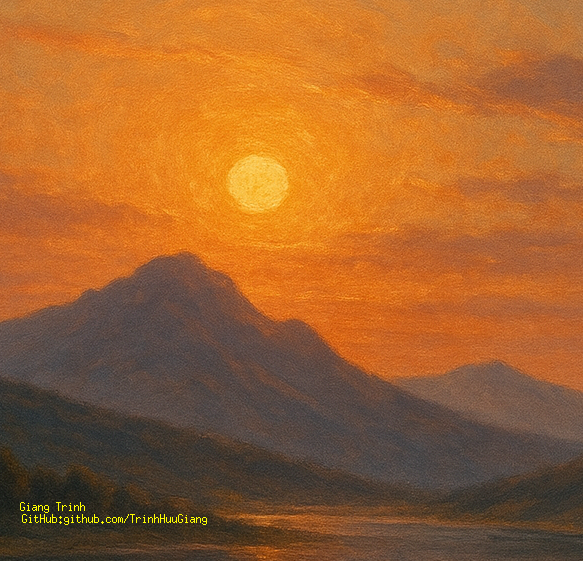
\includegraphics[width=5cm]{./sunset.png} \\
    \textbf{Hello\thanks{\LaTeX {} wikibook}}
}
\author{Giang Trinh\thanks{GitHub: \url{{https://github.com/TrinhHuuGiang}}}
    \and others\thanks{No one}}
\maketitle
%                            ================================
%                            Abstract
%                            ================================

%                            ================================
%                            Table of contents
%                            - TOC, LOF, LOT
%                            ================================
% \tableofcontents
% \listoftables
% \listoffigures


%                                                        ================================
%                                                        [Main matter]
%                                                        - Main topics
%                                                        ================================
\chapter{This is test chapter: math}

This is 2 plus implement by 2 displayed equation \verb` \{ \} `:
\[
\sum a+b = d + e + f
\]
\[
\sum b+d = a
\] \\

This is multiple mathematics, align by \textbf{`align' environment} depend on mark \verb|&|
\begin{align}
    \sum a+b &= d + e + f \label{eq: no1}  \\
    \sum b+d &= a \label{eq: no2}
\end{align}

This is mathematics auto numbering by \textbf{`equation'} environment
\begin{equation}
    \sum a+b = d + e + f \label{eq: no3}
\end{equation}

This is inline equation implement by \verb^ \( \) ^ : $ \sum a+b $ \\
\hspace{1cm}The $\sum$ seem smaller than above equations when not using \verb!\displaystyle! \\

This is inline equation implement by \verb^ \( \) ^ : $ \displaystyle  \sum a+b $ \\
\hspace{1cm}The $\sum$ seem similar with above equations when using \verb!\displaystyle! \\

Special symbol and functions:\\
\begin{enumerate}
    \item $\alpha, A, \beta, B, \gamma, \Gamma, \pi, \Pi, \phi, \Phi, \varphi, \mu$
    \item $\cos, \sin, \tan, \cot, \cosh, \sinh, \tanh, \coth$
    \item $a^{b+c} \; and \; i_{x+y} $
    \item $\lim_{a \to b} \; and \; \lim_{-\infty \to \infty}$
    \item $f(n) = n^5 + 4n^2 + 2|_{n=17}$
    \item $\forall \; and \; \subset \; and \; \in $
    \item $\frac{numerator}{denominator}$
    \item $\binom{n}{k}$
    \item $\frac{\frac{1}{x}+\frac{1}{y}}{y-z} \; or \; ^{numerator}/_{denominator}$
    \item $\sqrt{\frac{a}{b}} \;and \; \sqrt[n]{a}$
    \item $ \textbf{apple} \times 100 $
    \item $ \sum, \prod, \bigoplus, \bigotimes, \bigodot $
    \item $ \int, \iint ,\iiint, \oint, \idotsint, \vdots, \ldots, \cdots, \ddots, \mid, \nmid $
    \item $\sum_{
            \substack{
                0<i<m\\
                0<j<n}
                } P(i,j)$
    \item $( a ), [ b ], \{ c \},| d |, \| e \|, \langle f \rangle,
            \lfloor g \rfloor,  \lceil h \rceil , \ulcorner i \urcorner$
    \item $ \begin{matrix}
                a & b & c \\
                d & e & f \\
                g & h & i
            \end{matrix} $

\end{enumerate}

This is \verb|\frac|
\begin{equation}
x = a_0 + \frac{1}{a_1
+ \frac{1}{a_2
+ \frac{1}{a_3 + \frac{1}{a_4} } } }
\end{equation}

This is \verb|\cfrac|
\begin{equation}
x = a_0 + \cfrac{1}{a_1
+ \cfrac{1}{a_2
+ \cfrac{1}{a_3 + \cfrac{1}{a_4} } } }
\end{equation}


% code
\chapter{This is test chapter: Code}

\lstinputlisting[language=C,
        numbers=left, firstnumber=10, stepnumber=2]{./sample.c}


%                                                        ================================
%                                                        Appendix
%                                                        - Subordinate chapters
%                                                        ================================

%                                                        ================================
%                                                        Back matter
%                                                        - Bibliography
%                                                        - Glossary/Index
%                                                        ================================





%                            ================================
%                            END
%                            ================================
\end{document}

